\section{Introduction}
In the past year, language models such as CodeLlama \citep{roziere2023code}, DeepSeek-Coder \citep{guo2024deepseek}, and GPT-4 \citep{openai2023gpt} have demonstrated great advances in code generation. Their success has primarily been due to their strong code generation abilities, as measured by benchmarks such as HumanEval \citep{chen2021evaluating} and MBPP \citep{austin2021program} as well as their usefulness in general-purpose code writing. While these models are able to produce correct code for impressively complex specifications, they just as often produce incorrect code.

Some of these incorrect programs contain egregious mistakes, but others fail in more subtle ways. We focus our attention towards the second group, which we call \textit{\textbf{counterfeit samples}}. We define a counterfeit sample to be a program sampled from a code language model which is 1) good enough to be generated by the language model at a moderate temperature, 2) are incorrect, and 3) pass weak but nontrivial correctness checks. In this work, we study the extent to which models can understand these counterfeit programs. This final criterion of passing nontrivial correctness checks distinguishes programs with more subtle errors from those that trivially fail and are likely uninteresting. In Fig. \ref{fig:main}, we show an example of an incorrect, counterfeit, and correct program. Because we use relatively weak correctness checks, many counterfeit programs can still be easily detected as wrong by a human.

\begin{figure*}[ht!]
    \centering
    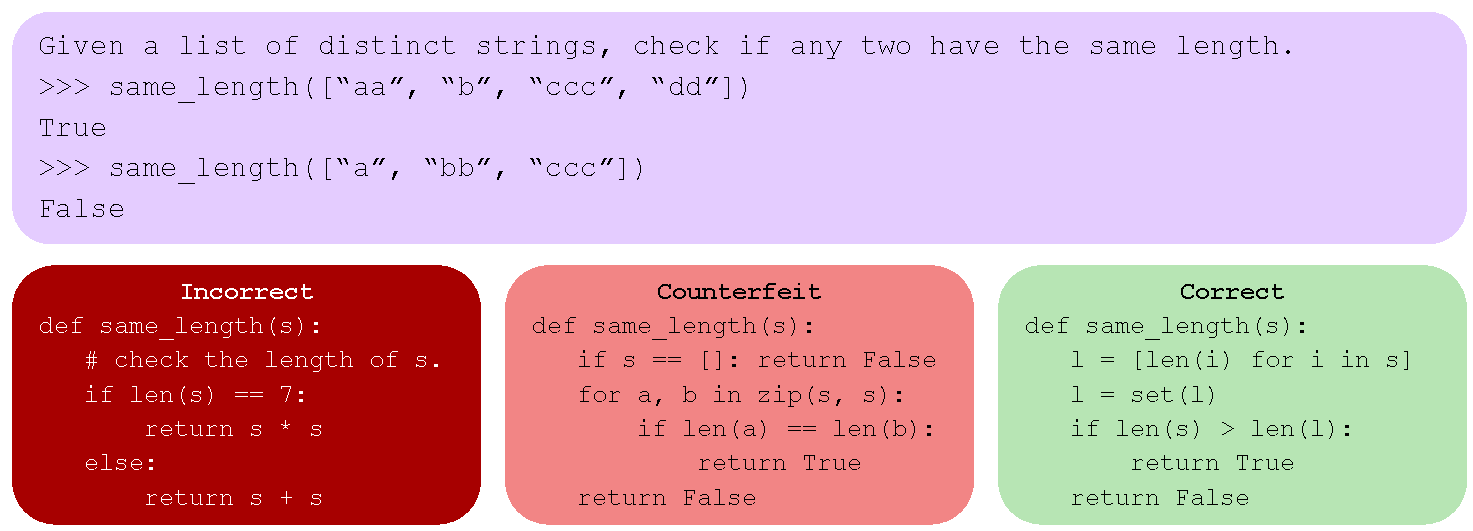
\includegraphics[width=0.95\textwidth]{figures_v2/main/misc/fig1.pdf}
    \caption{Example of a problem specification with incorrect, counterfeit, and correct programs.}
    \label{fig:main}
\end{figure*}

We provide empirical evidence that code language models have a shallow understanding of these counterfeit samples (Sec. \ref{sec:understanding-counterfeit}) via three evaluations: correctness checking, execution prediction, and program repair. For correctness checking, the model is asked to assess whether a short piece of code correctly implements a natural language specification (sometimes with test cases). For execution prediction, the model is given a program-input pair and asked to predict the output of executing the program on the given input. For fairness, we ensure the programs are generally short and that execution does not require complex calculations. For repair, the model is given the counterfeit program alongside its original specification and is asked to correct it. First, we find that models frequently misjudge counterfeit samples as correct. Second, models are much worse at reasoning about the execution of counterfeits than their correct companions, often executing counterfeits as if their semantics matched those of a correct program. Third, models falter at repair: the likelihood of a model successfully repairing a counterfeit example is often even lower than that of generating a correct program when sampling from scratch. As a caveat, this paper focuses on open-source models, primarily CodeLlama 34B and DeepSeek Instruct 33B. We also present limited results on GPT-3.5 and GPT-4 which suggest that GPT-3.5 behaves similarly to the open-source models while GPT-4 has a much better understanding of counterfeits. Nevertheless, we still find that GPT-4 still exhibits some of these misunderstandings.

Through further analysis, we find that counterfeit samples have other unexpected properties
(Sec. \ref{sec:analyzing-counterfeit}). We find, for example, that counterfeit samples from problems that are easier for the model to solve are \textit{not} easier to assess and only slightly easier to execute and repair, highlighting an inconsistency between generation and understanding capabilities. We also observe that models don't perceive their own counterfeit samples differently from other models' counterfeits and that models of all capability levels are able to generate equally difficult counterfeit samples.

Overall, we find that these counterfeit samples are, in a sense, adversarial to the model: models often struggle to assess their correctness, reason about their execution as if they were correct programs, and repair them at a low rate. Understanding counterfeit samples is a prerequisite to many downstream applications in which models use their own feedback to improve themselves. Therefore, in light of our findings, we recommend exercising caution in these schemes such as self-repair and model-based reranking of outputs, especially when no external feedback is incorporated.